\section{Introduction}
\label{sec:introduction}
The high-speed development of social networks brings explosive scale of information. The convenience of the social networks accelerates the diffusion of information. People create and publish messages without any limitations, which leads to the widespread dissemination of rumors in social networks \cite{DBLP:journals/corr/KurkaGZ15, DBLP:journals/csur/ZubiagaABLP18, DBLP:conf/sirocco/KostkaOW08, vosoughi2018spread}. Rumors usually appear with unjudged veracity and contain substantive misinformation, which may cause huge damage to the society. For instance, a large number of rumors arise during the COVID-19 epidemic, such as ``More than ten thousand people die in Wuhan." and ``Liquor kills the virus.", causing great public panic. Therefore, it is an urgent task to defeat rumors in social networks.

Social media generates huge amounts of data all the time. It is impracticable to manually defeat rumors on this numerous data. Therefore, many studies have been carried out to automatically defeat rumors and the contributions are divided into two categories: diffusion-based rumor source identification and content-based rumor detection. Diffusion-based rumor source identification aims to locate the sources of the rumor at the early stage of rumor diffusion \cite{DBLP:conf/sigmetrics/ShahZ10, DBLP:journals/tit/ShahZ11, DBLP:conf/kdd/LappasTGM10}. Content-based rumor detection aims to judge the veracity of tweet sequences. As shown in Fig.\ref{fig:pipeline}, this task is a pipeline that is divided into four sub-tasks \cite{DBLP:journals/csur/ZubiagaABLP18, DBLP:conf/coling/KochkinaLZ18}: rumor detection, rumor tracking, sentence classification, and veracity. Rumor detection is to determine whether a tweet sequence is a rumor  \cite{DBLP:conf/socinfo/ZubiagaLP17, DBLP:conf/www/Ma0W19,DBLP:conf/naacl/NguyenDCD19, DBLP:journals/corr/abs-1906-05659}. Sentence classification is to judge the emotion of a tweet sentence \cite{DBLP:conf/semeval/EnayetE17, DBLP:conf/semeval/X17a, DBLP:conf/coling/ZubiagaKLPL16}. Rumor veracity is to determine if a tweet tells the truth \cite{DBLP:conf/coling/KochkinaLZ18, DBLP:conf/acl/LiZS19, DBLP:conf/acl/KumarC19}. These three sub-tasks have attracted extensive attention in recent years. However, only a few studies have been proposed for the rumor tracking task.

Rumor tracking is to collect relevant tweets of a given rumor event. It can be considered to a binary classification problem that classifies the posts to be related or unrelated. However, the existing proposals \cite{DBLP:conf/emnlp/QazvinianRRM11, DBLP:conf/www/ChengNB20}  only consider rumor tracking as an auxiliary task in multi-task learning without special optimization, hence restraining the accuracy of tracking performance.
Therefore, we propose a model that improves the weakness of the existing work for rumor tracking.

The main contributions of this work are summarized as follows:
\begin{itemize}
	\item By exploring plenty of basic models, we proposed an aggregated model named RL-BRT to solve the rumor tracking task. 
	\item We analyze the rumor tracking task and find suitable features and embedding methods. Also, we propose a reinforcement learning based bagging algorithm to aggregate basic models into a macrocosm.
	\item We conduct experiments on public benchmark datasets, and the experimental results show the rationality and superiority of RL-BRT.
\end{itemize}

The rest of this article is structured as follows. In Section \ref{sec:related}, we introduce important works related to RL-BRT. In Section \ref{sec:perliminary}, we introduce some notations and background knowledge of this work. Our proposed model RL-BRT is introduced in Section \ref{sec:model}. Then, Section \ref{sec:experiment} shows the experimental settings and results. Finally, we give the conclusion and future work in Section \ref{sec:conclusion}.

\begin{figure}[tbp]
	\hspace{0ex}
	\vspace{0ex}
	\centering
	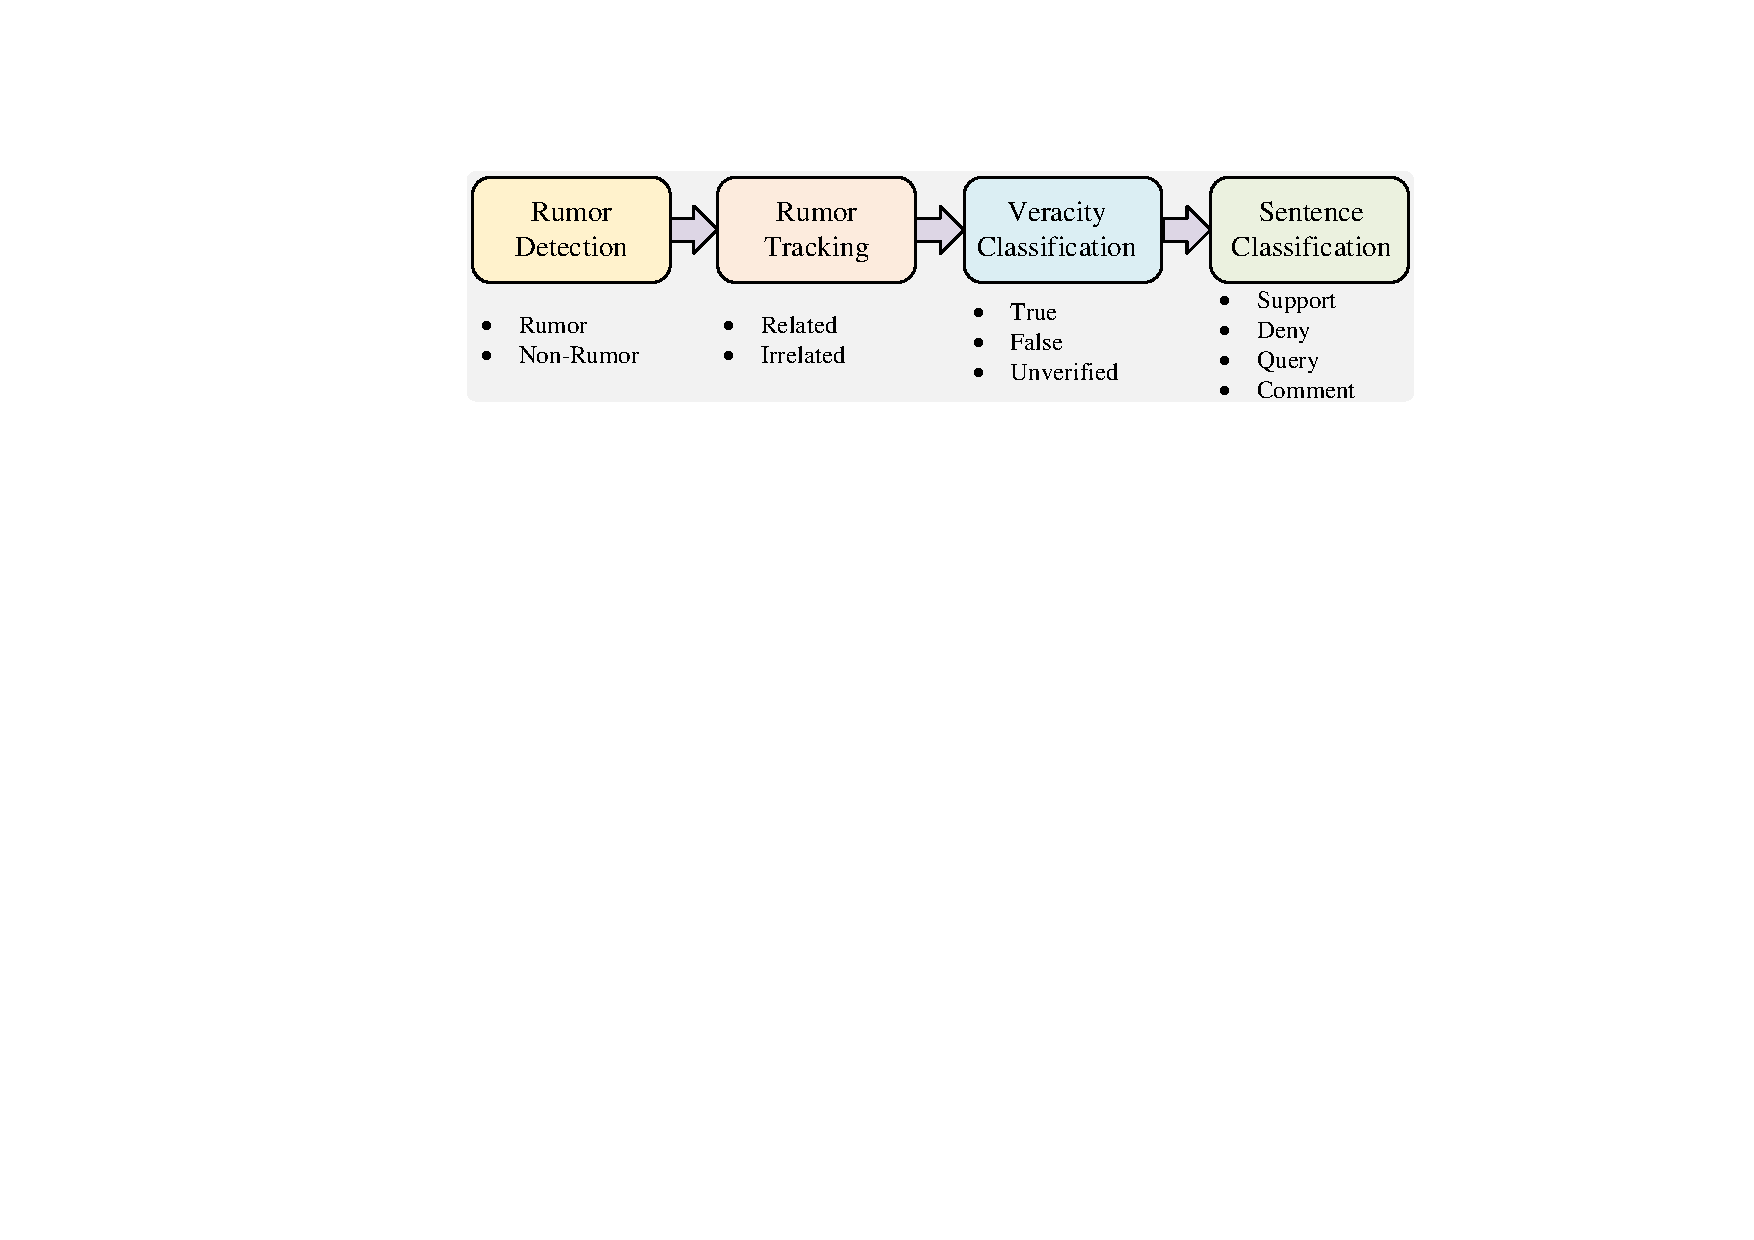
\includegraphics[width = \textwidth]{fig/pipeline}
	\caption{Pipeline of Rumor Detection Task}
	\label{fig:pipeline}
\end{figure}